\documentclass[10pt, pscyr, nonums]{hedlabwork}
\usepackage[russian]{babel}
\usepackage{hedmaths}
\usepackage{hedphysics}
\usepackage{graphicx}
\graphicspath{{images/}, {plots/}}

\newgeometry{top=1.5cm, bottom=1.5cm, left=1cm, right=1cm}

\student{} \date{}
\labnum{601}
\labname{Определение электродвижущей силы термопары}

\begin{document}
  \makeheader

  \emph{Цель работы:} определение зависимости термоэлектродвижущей силы
  термопары от разности температур спаев.

  \emph{Используемые при расчетах формулы и значения:}
  \( \EMF_T = \alpha (T_2 - T_1) \), \( \Delta T = T_2 - T_1 \).

  \begin{figure}[h!]
    \center
    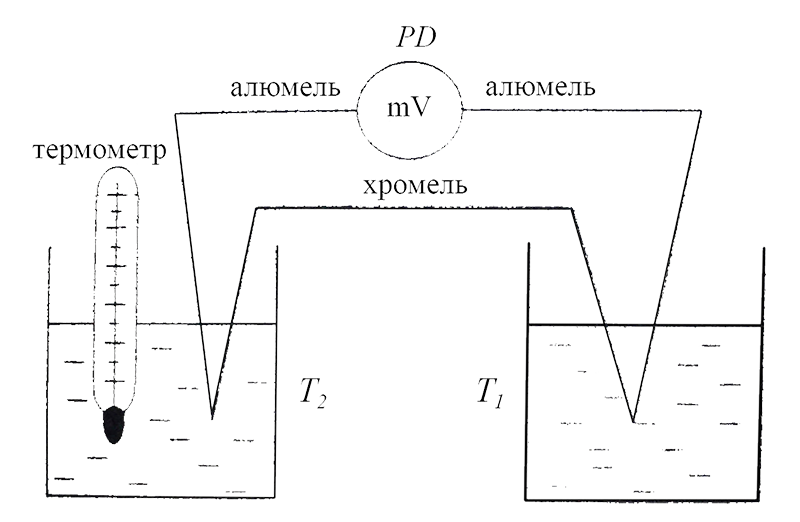
\includegraphics[width=.5\textwidth]{appearance} \\
    \parbox{.5\textwidth}{\caption{Внешний вид установки}}
  \end{figure}
  \vspace*{-2em}

  \begin{table}[h!]
    \center \caption{Результаты измерений}
    \begin{tabular}{|*{5}{C{.12}|}} \hline
      \( T_1 \), К & \( T_2 \), К & \( \Delta T \), К &
        \( \EMF_T \), В & \( \alpha \), В/К \\ \hline
      \multirow{10}{*}{} &&&& \multirow{10}{*}{} \\ \cline{2-4}
      &&&& \\ \cline{2-4}
      &&&& \\ \cline{2-4}
      &&&& \\ \cline{2-4}
      &&&& \\ \cline{2-4}
      &&&& \\ \cline{2-4}
      &&&& \\ \cline{2-4}
      &&&& \\ \cline{2-4}
      &&&& \\ \cline{2-4}
      &&&& \\ \hline
    \end{tabular}
  \end{table}

  \subsection{Подсчет погрешности и окончательные результаты}
  \center
  \rule{.95\textwidth}{.5pt} \\ \rule{.95\textwidth}{.5pt}
  \rule{.95\textwidth}{.5pt} \\ \rule{.95\textwidth}{.5pt}
  \rule{.95\textwidth}{.5pt} \\ \rule{.95\textwidth}{.5pt}
  \rule{.95\textwidth}{.5pt} \\ \rule{.95\textwidth}{.5pt}
  \rule{.95\textwidth}{.5pt} \\ \vspace*{2em}

  \emph{Вывод:} \rule{.885\textwidth}{.5pt}
  \rule{.95\textwidth}{.5pt} \\ \rule{.95\textwidth}{.5pt}
\end{document}
